% Template for ICME 2018 paper; to be used with:
%          spconf.sty  - ICASSP/ICIP/ICME LaTeX style file, and
%          IEEEbib.bst - IEEE bibliography style file.
% --------------------------------------------------------------------------
\documentclass{article}
\usepackage{spconf,amsmath,epsfig}
\usepackage{graphicx}
\usepackage{subfigure}
\pagestyle{empty}

\usepackage{color}


\definecolor{red}{rgb}{1.0,0.0,0.0}
\definecolor{blue}{rgb}{0.0,0.0,1.0}
\definecolor{purple}{rgb}{0.5,0.0,0.5}


\newcommand{\comments}[1]{}
\newcommand{\xj}[1]{\textcolor{red}{(xuejin:#1)}}
\newcommand{\md}[1]{\textcolor{purple}{#1}} 
\newcommand{\camin} {\mathbf{K}}
\newcommand{\camex}{\mathbf{M}}
\newcommand{\vb}[1]{\mathbf{#1}}



\begin{document}\sloppy

% Example definitions.
% --------------------
\def\x{{\mathbf x}}
\def\L{{\cal L}}


% Title.
% ------
\title{A Hybrid System Integrating Calibration and Registration for Accurate 3D Reconstruction}
%
% Single address.
% ---------------
\name{Paper 1375}
\address{ }


\maketitle


%
\begin{abstract}
With the development of virtual and augmented reality, 3D reconstruction for indoor scenes based on multi-camera systems has become increasingly popular recently. 
%
The quality of reconstructions from images relies on many factors, including the multi-view camera calibration accuracy and the depth estimation quality in each single view. 
%
In this paper, we propose a hybrid system which integrates a global camera parameter estimation and 3D registration instead of traditional pairwise framework, to produce low-error point cloud models.
%replace the traditional pairwise relations of both camera and model fusion to a global framework. 
%
First, a global bundle adjustment is adopted to increase the accuracy of camera pose estimation. 
%We use checkerboard corners to optimize the camera extrinsic parameters globally which are obtained by pairwise camera calibration methods. 
Second, a point cloud registration is used to fuse the inaccurate depth maps to a 3D model. 
We use the Iterative Closest Point (ICP) algorithm to register the point clouds estimated from different views to minimize the model deviation. 
The experimental results show the promising effect of our method to produce high-quality models.
\end{abstract}
%
\begin{keywords}
Multi-camera system, 3D reconstruction, camera calibration, point cloud registration
\end{keywords}
%

\section{Introduction}
Indoor 3D reconstruction from multiple views has become more and more prevalent in recent years~\cite{dou2016fusion4d,orts2016holoportation}. High-quality reconstruction has bright future in many applications like telecommunication and VR Games. Compared with the systems based on a single camera, multi-camera systems using RGB cameras have many advantages such as a wider horizon. Meanwhile, to achieve high-quality results, other kinds of sensors are also widely used in the reconstruction system, such as Near Infra-Red (NIR) cameras to estimate depth maps. Hence, the quality of the final reconstruction result depends on many aspects in a multi-camera system, especially on the accuracy of the camera parameters and depth maps.

For a single camera, its intrinsic parameters can be accurately estimated by many internal calibration techniques~\cite{zhang2000flexible,zhang2004camera}.
For multi-camera calibration, a series of approaches have been proposed as well.
One widely used technique for accurate calibration is to use specialized calibration objects, such as planar patterns, rig and so on.
%
Li et al. proposed a specially designed calibration pattern for feature detection and accurate matching~\cite{Li2013A}. %The pattern can be automatically detected even if the pattern is partially visible in an image.
This method works well especially on the systems with a few cameras with small overlapping fields of view.
%
Zhao and Liu proposed an algorithm based on 1D objects for a triple camera system~\cite{zhao2008practical}.
A 20cm-long stick with 3 markers rotating around a fixed point is used as the calibration object.
The algorithm integrates a rank-4 factorization with the standard 1D camera calibration method and is much more convenient than plane-based algorithms.
Svoboda et al. proposed a method that only requires a bright-spot object like a laser pointer~\cite{svoboda2005convenient}.
Waving the object which can be easily detected in each image through the working space is the only work requested.
%
Kalibr~\cite{Maye2013Self} is a free toolbox that solves the multiple camera calibration problem using special 2D barcodes by calibrating neighboring cameras those have overlapping fields of view.
%It could produce a good estimate but requires that neighboring cameras have overlapping fields of view. \xj{Every calibration system requires overlapping regions..}
%However, if the system contains many cameras those do not share the same overlapping fields of view, the calibration process should be simply repeated for each pair of cameras.
%
However, repeating the sequential calibration process results in accumulated errors.
%
Liu et al.~\cite{Liu2015Algorithm} proposed an algorithm for camera parameter adjustment using a checkerboard. They divide a four-camera system into six two-camera subsystems. With a vertically placed checkerboard which is printed on two sides, the corners can be seen in each subsystem and the global adjustment can be done.
However, if there are more cameras in the system, it is hard for all the cameras to capture a checkerboard at the same time due to the oblique angle.


Another category of multi-camera calibration techniques is self-calibration, which does not require any specialized objects.
However these methods are very sensitive to the textures in the captured scene and usually suffer from the low accuracy.
%
Bundler~\cite{snavely2006photo} is a structure-from-motion technique to simultaneously estimate the camera parameters and the 3D point positions from a set of unordered images.
%
It uses SIFT keypoint detector~\cite{lowe2004distinctive} which works well on outdoor scenes but typically fails to find enough point correspondences in indoor cases.
%
Vasconcelos et al.~\cite{vasconcelos2012minimal} proposed a solution to calibrate a camera with two other calibrated cameras.
Bushnevskiy et al.~\cite{bushnevskiy2016multicamera} presented a novel approach that enforces constraints arising from the visible epipoles and is especially suitable for dome-like indoor cases.

All these methods use RGB images to calibrate multi-camera systems.
%
Besides of camera parameters, another important influencing factor to the final reconstruction is the depth estimation of each view.
Intensive research has been done on the depth estimation problem~\cite{scharstein,Bleyer2011PatchMatch}, whereas the error can not be eliminated entirely.
%
Rather than to improve the quality of depth estimation, we use a 3D registration step to diminish the influence of the depth errors in the fused 3D model.
%
A lot of work has been done in the registration of point sets.
Iterative Closest Point (ICP)~\cite{Besl1992A} is the most popular registration method, which performs well with proper initialization.
%
Many registration methods which do not rely on the starting positions of the point clouds have also been proposed~\cite{Aiger:2008:CSR:1360612.1360684,5152473}.
%
For multiple point-set registration, different from using the sequential pairwise registration strategy, Evangelidis et al.~\cite{Evangelidis-ECCV-2014} proposed a method that treats all the point clouds on equal terms, and register multiple point clouds globally.
%
%They use a generative model and the registration is converted to a clustering problem.
%
However, if two point clouds from different views have the similar shape, for example, the point clouds of the front and the back of a human body, the two point clouds may totally overlap after the registration, which leads to a wrong result.
This problem can be solved using the correspondences between the point clouds from the neighboring views by sequential registration.
%

In this paper, we present a hybrid system integrating both calibration and registration to achieve high-quality reconstruction results. To avoid the accumulative error caused by the repetitive calibration for each pair of cameras, we use a global camera calibration method.
Afterwards, we use the point cloud registration method to register the partial point clouds generated from all views.
This can effectively reduce the impact of the error in depth estimation and obtain a high-quality 3D reconstruction.







\section{Algorithm}
\label{sec:overview}

\xj{I add the problem definition here.}


%\textbf{Problem Definition.}
A multi-camera system is set up to capture objects in an indoor scene, as shown in Fig.~\ref{fig:rig}.
%The cameras in our 3D reconstruction system are placed on the periphery of the room pointing inwards, only the neighboring cameras have overlapping fields of view. \xj{what is the point of this overlapping fov?}
%
$K$ ($K=8$) camera pods are installed around the working space looking inwards for a full capture.
Each camera pod consists of one color camera and two Near Infra-Red cameras. A laser pointer is used to produce special patterns. From the pair of images of the projected patterns captured by the two NIR cameras, a depth map $D_k$ can be estimated using PatchMatch stereo algorithm~\cite{Bleyer2011PatchMatch}.
There are also several alternative depth cameras or depth estimation algorithm to obtain the depth map of each view. Most of them produce a rough depth map with noise and errors.
As Fig.~\ref{fig:deptherror} shows, the estimated depth map encounters large distortions on the boundary of the human body, and missing data in the head area.
How to improve the quality of depth map is beyond the scope of this paper.

\begin{figure}
	\centering
	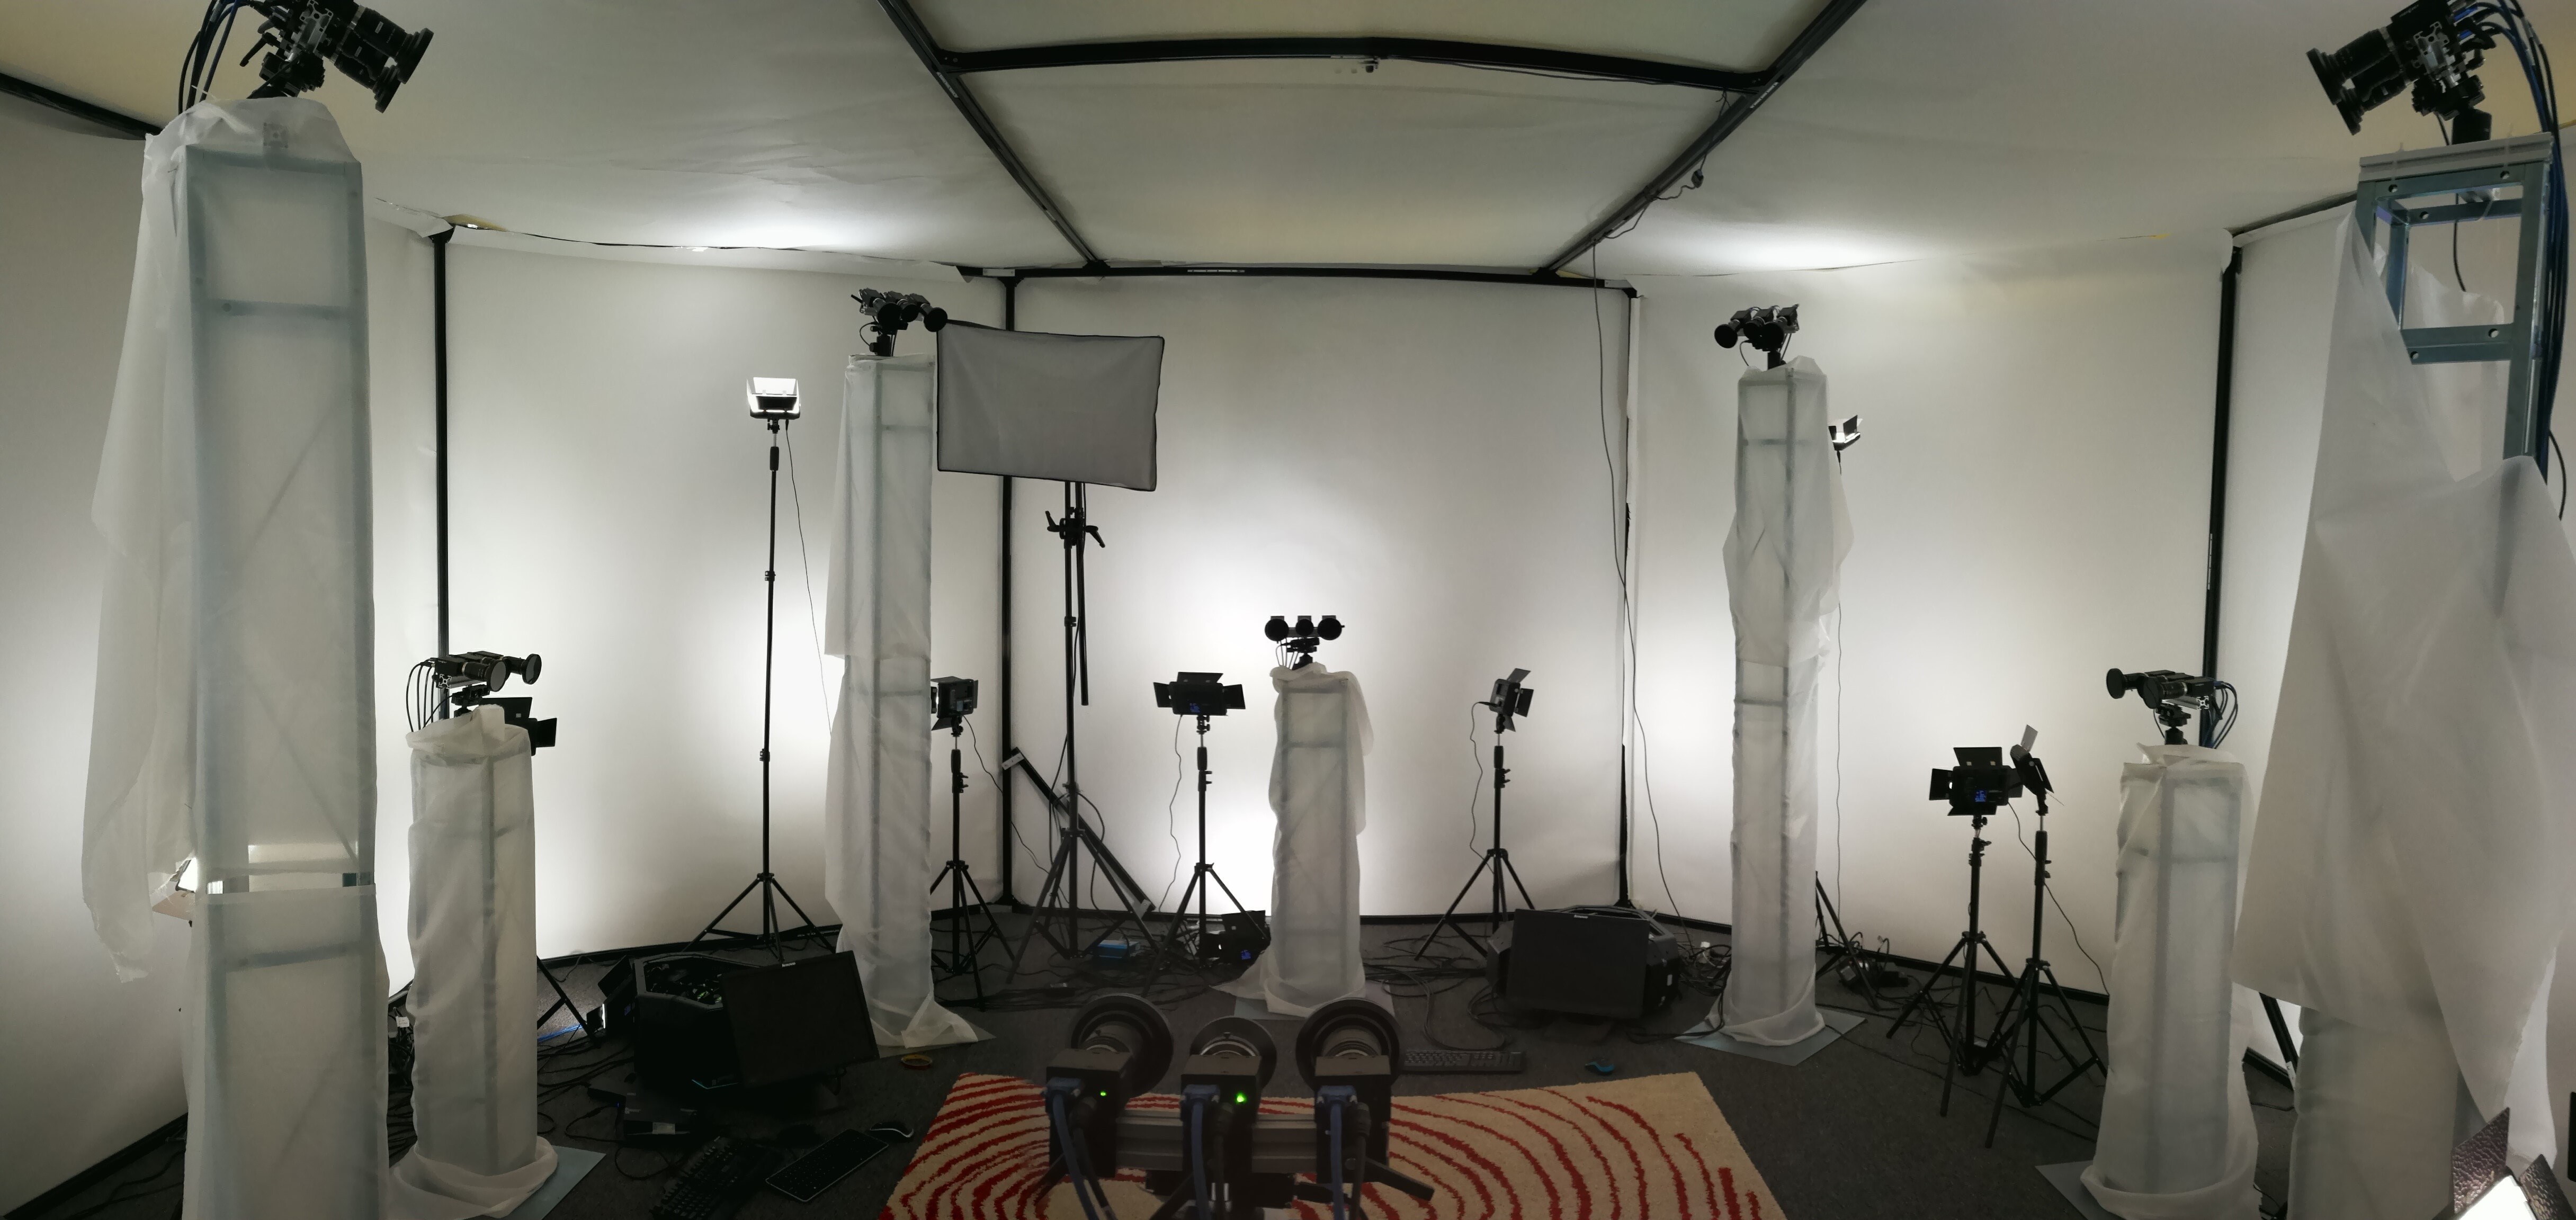
\includegraphics[width=\columnwidth]{image/rig.jpg}
	\caption{Our multi-camera system with 8 camera pods pointing inwards.}
	\label{fig:rig}
\end{figure}



\begin{figure*}[ht]
	\centering
	\subfigure[]{
		\begin{minipage}[c]{.22\linewidth}
			\centering
			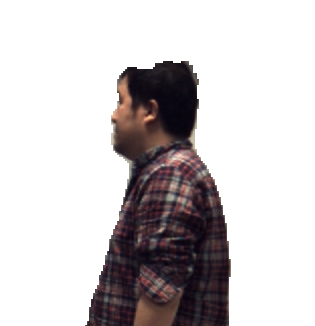
\includegraphics[width=4cm]{image/depth_error_rgb.png}
		\end{minipage}
	}%
	\subfigure[]{
		\begin{minipage}[c]{.22\linewidth}
			\centering
			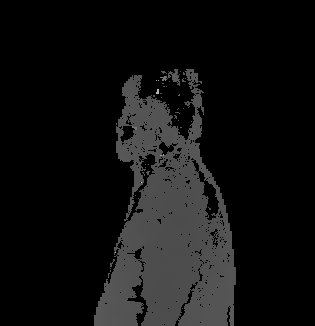
\includegraphics[width=4cm]{image/depth_error_depth.png}
		\end{minipage}
	}
	\subfigure[]{
		\begin{minipage}[c]{.22\linewidth}
			\centering
			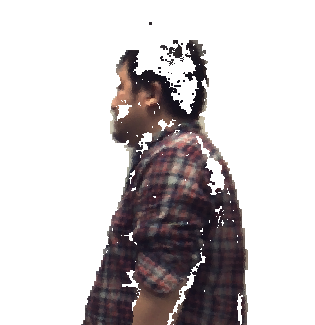
\includegraphics[width=4cm]{image/depth_error_pc.png}
		\end{minipage}
	}
	\subfigure[]{
		\begin{minipage}[c]{.22\linewidth}
			\centering
			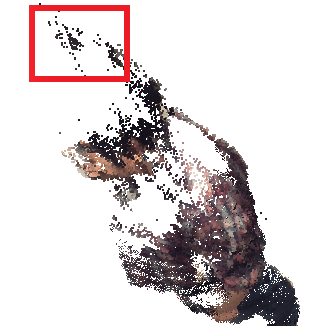
\includegraphics[width=4cm]{image/depth_error_pc_2.png}
		\end{minipage}
	}
	\caption{Errors in depth estimation. (a) RGB; (b) Depth; (c) The point cloud reconstructed from RGBD data. (d) Another view of the point cloud. The distortion of the head region (in the red box) is caused by the inaccurate depth estimation. }
	\label{fig:deptherror}
\end{figure*}



%
Under the assumption of pinhole camera, each camera has a group of parameters including the intrinsic matrix $K$ and extrinsic matrix $M$ to project a point $P$ in the 3D space to its image plane as
\begin{equation}\label{eq:cam-proj}
z_{p}\mathbf{x}=\mathbf{K}\mathbf{M}\mathbf{p},
\end{equation}
where $\mathbf{p}=(x,y,z,1)^{T}$ is the homogeneous coordinate of $P$, and $\mathbf{x}=(u,v,1)^{T}$ is the homogeneous coordinate of its projected point on the image plane.
%


From the depth map estimated by each camera pod, a partial point cloud can be reconstructed by back-projecting each pixel in the depth map into the 3D space according to the pose parameters of each camera.
%
A 3D model can be obtained by fusing the $K$ point clouds.
%
%
Ideally, with the accurate depth $z_p$ of each image point $\vb{x}$, and accurate camera parameters $\camin$ and $\camex$, the image pixels captured in different views can be back-projected to the 3D space and well aligned to a 3D point $\vb{p}$.
%
However, due to the unavoidable error and noises in depth maps, our framework relies on two main parts to reconstruct a high-quality model.
%
The first part is a global camera calibration method to estimate the camera parameters $\{\camin_k, \camex_k\}^{K}_{k=1}$ as accurate as possible, as described in Sec.~\ref{sec:global-calib}.
The second is a registration method to produce 3D point clouds as consistent as possible from in-accurate depth $z_p$, as described in Sec.~\ref{sec:registration}.
\xj{Explain with a pipeline figure.}
\md{To Do}




\comments{

Our algorithm consists of two main parts. Firstly, we use the toolbox Kalibr~\cite{Maye2013Self} to calibrate our multi-camera system and achieve the intrinsic and initial extrinsic parameters of all our cameras. Then we use a checkerboard as the calibration object, detect the corners on it and do the global extrinsic parameters optimization, as described in Sec.~\ref{sec:global-calib}.
%
Secondly, we use the camera parameters and the input RGB and depth images to reconstruct the point clouds of the model and use ICP (Iterative Closest Point)~\cite{Besl1992A} to align the point clouds of different views.
With the transform of the registration, the error caused by depth estimation can be minimized and a more accurate 3D reconstruction can be achieved, as described in Sec.~\ref{sec:registration}.
Finally, we compare the reconstruction results using different methods. We also compute the reprojection error and use a plaster model as the ground truth to verify the effectivity of our algorithm, as described in Sec.~\ref{sec:Results}.
\xj{Show a system pipeline.}
}
 


\section{Global Camera Calibration}
\label{sec:algorithm}

\xj{Need a paragraph or section to describe the whole system of generating the final 3D model.}


The cameras in our 3D reconstruction system are placed on the periphery of the room pointing inwards, only the neighboring cameras have overlapping fields of view. We found that if we calibrate the cameras pairwisely, accumulative error will occur and can be seen obviously in the result of the reconstruction. After the initial calibration, \xj{what is the input and output of the initial calibration?} we optimize the extrinsic parameters globally using a checkerboard.

%\subsection{Multi-camera system}
\begin{figure*}[!htp]
\centering
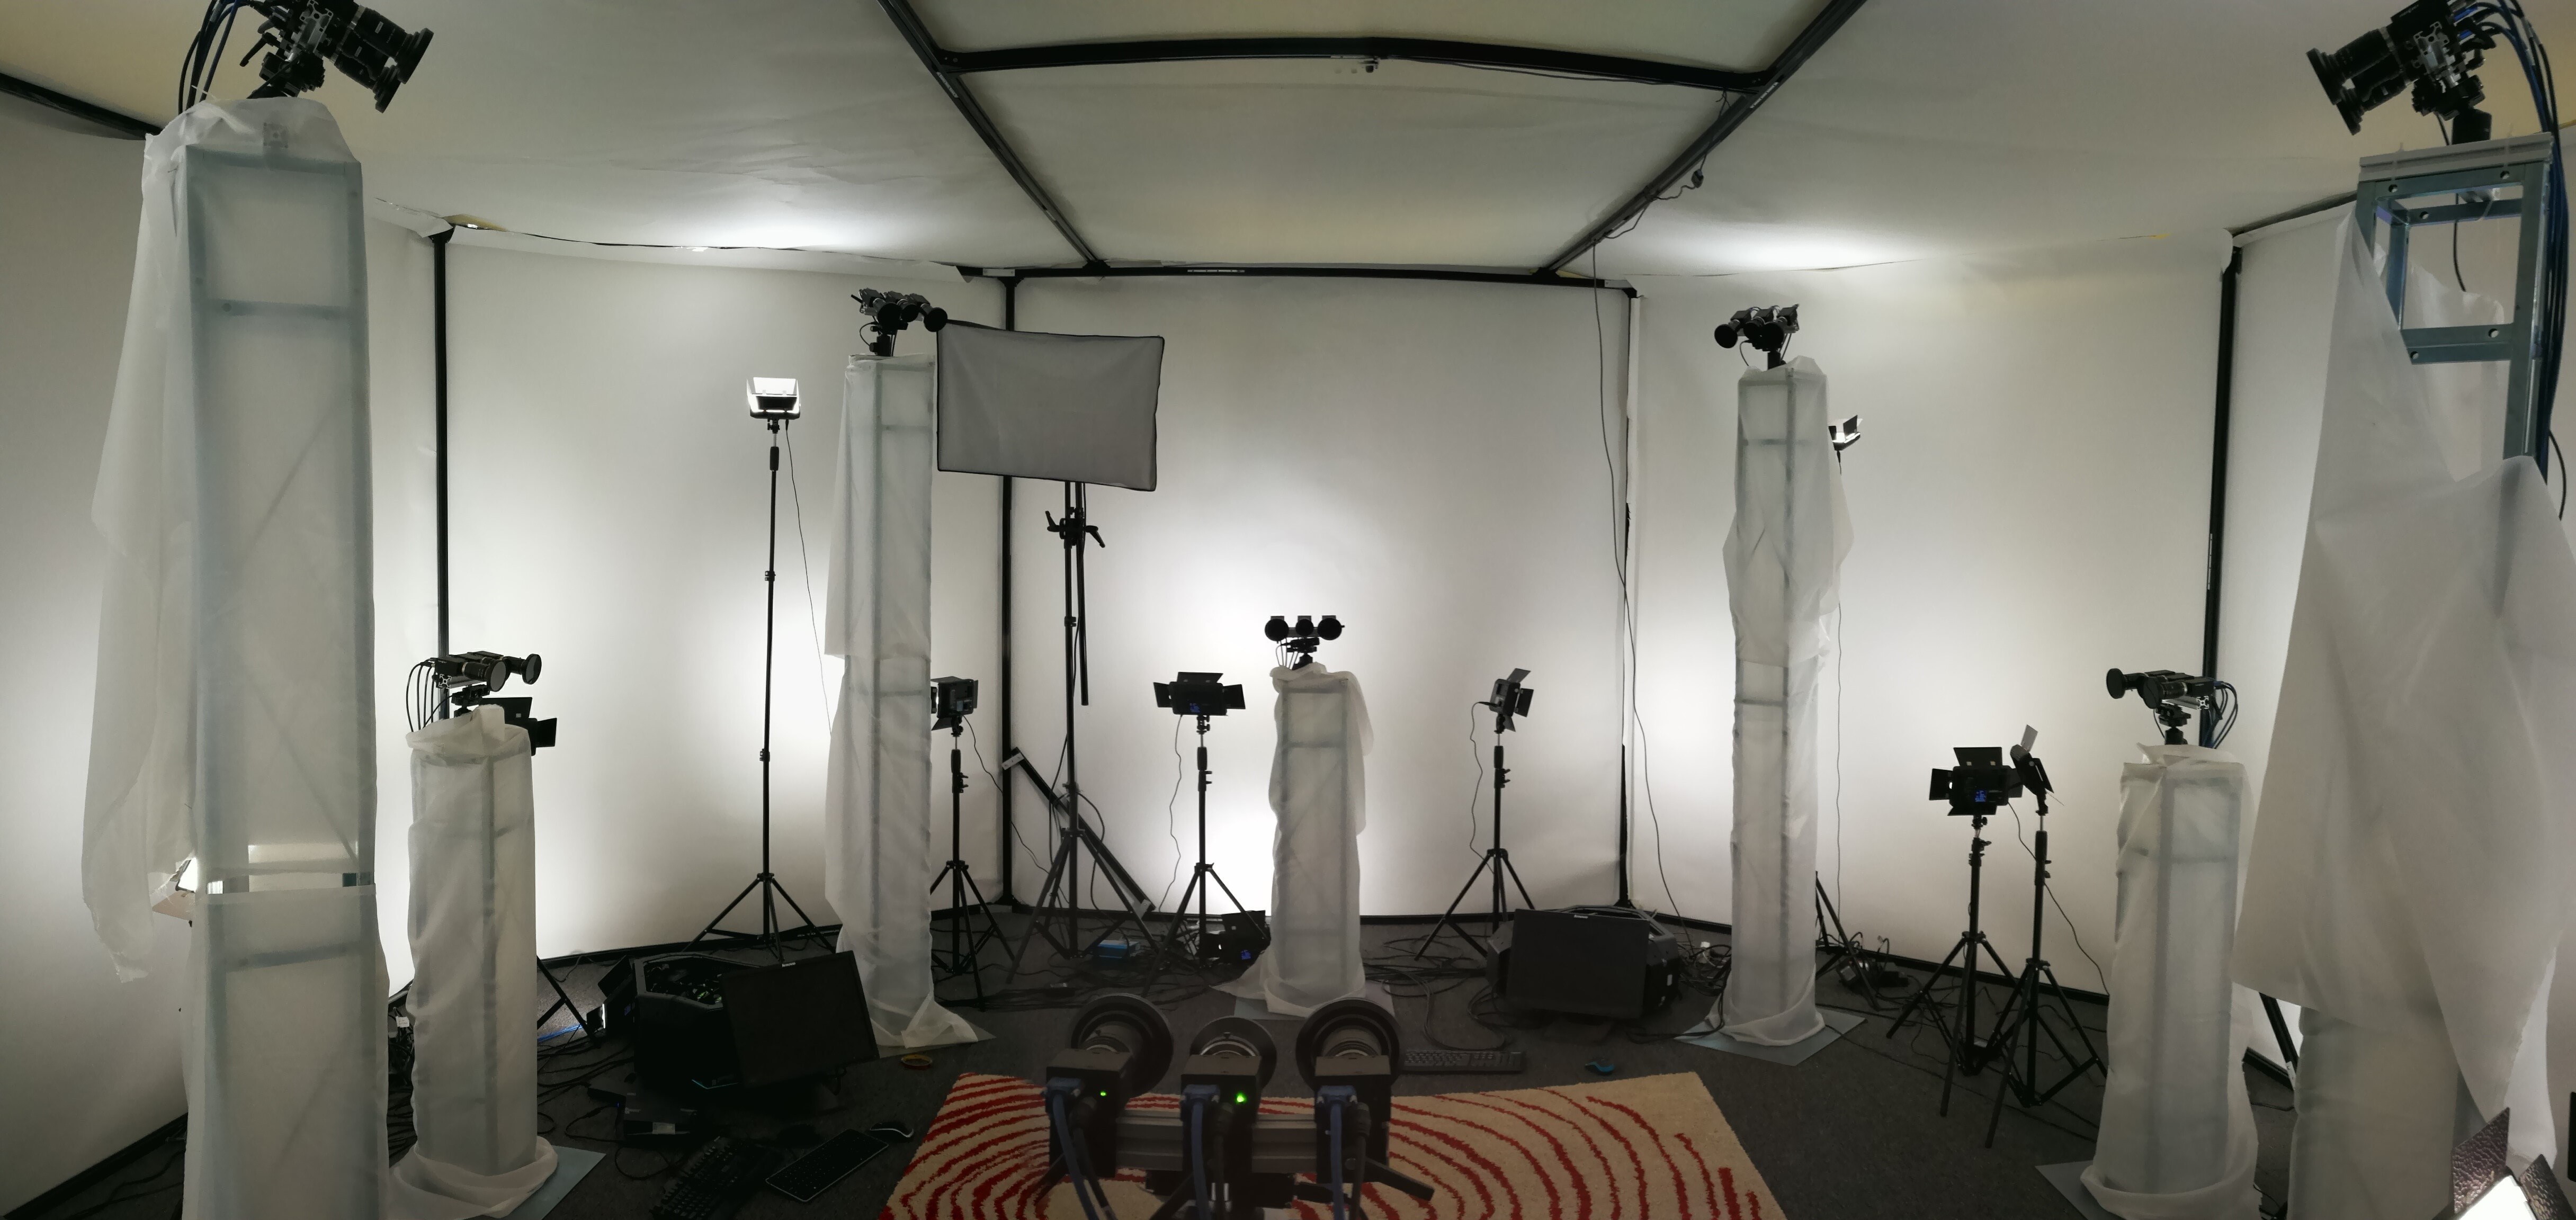
\includegraphics[scale=0.08]{image/rig.jpg}
\caption{Our multi-camera system with 8 camera pods pointing inwards.}
\label{fig:rig}
\end{figure*}

We employ 8 camera pods around the working space looking inwards for a full capture as shown in Figure~\ref{fig:rig}. Each camera pod consists of one color camera and two Near Infra-Red cameras. A laser pointer is used to produce special patterns.
From the two images of the projected patterns captured by the two NIR cameras, a depth map can be estimated using \xj{what algorithm?}
% it depth images can be achieved by the 2  using depth estimation methods.


%\subsection{Camera model}
Let $\mathbf{p}=(x,y,z,1)^{T}$ be the homogeneous coordinate of a point $P$ in the 3D space, and $\mathbf{x}=(u,v,1)^{T}$ the homogeneous coordinates of its projected point on an image plane, the perspective projection of a pin-hole camera is usually described as
\begin{equation}
z_{p}\mathbf{x}=\mathbf{K}\mathbf{M}\mathbf{p},
\end{equation}
where $z_{p}$ is the projective depth of point $P$, $\mathbf{K}$ and $\mathbf{M}$ are the intrinsic and extrinsic parameters of the camera.

%\subsection{Initial calibration}
The $\mathbf{K}$ and initial $\mathbf{M}$ of each camera are calibrated by Kalibr~\cite{Maye2013Self} pairwisely because of the lack of the common overlapping fields of view, including the 8 color cameras' extrinsic parameters $\{\mathbf{M}_{i}\}_{i=1,...,8}$. The extrinsic parameters from the 2 NIR cameras to the color camera in the same camera pod are also achieved, but these extrinsic parameters are fixed and used to estimate the depth in each view.

%\subsection{Global optimization}

We use a $6\times7$ checkerboard with squares of 117 mm for the optimization. 
\xj{Why do you need checkerboard? Why do you use 6x7 rather than other pattern?}
%
The user is requested to move the checkerboard in front of the cameras freely in the working space. The checkerboard can be simultaneously seen in three or four views usually. 
%
Then the 42 corners on the checkerboard can be detected in each group. 
%
We can estimate the 3D coordinates $\mathbf{P_{c}}$ of each corner from the corresponding 2D coordinates $\{\mathbf{p_{c}}_{j}\}_{j=1,...,n}$ by triangulation, where $n$ is the number of the views that the checkerboard can be seen in at the same time. 
To make the optimization result be more consistent to the whole system, we also use the images with checkerboard on the ground which allows the checkerboard corners can be seen in all the 8 cameras,  as shown in Figure~\ref{fig:checkerboard}. This will help to reduce the accumulative error and inconsistence caused by the pairwise calibration. 
The aim of the optimization is to minimize the sum of all reprojection errors with respect to all 3D points and extrinsic parameters, which is described as
\begin{equation}
E(\{\mathbf{K_{ex}}_{i}\})=\sum_{i}\sum_{j}((\mathbf{K_{in}}_{i}\mathbf{K_{ex}}_{i}\mathbf{P_{c}}_{j})-\mathbf{p_{c}}_{ij})^{2}.
\end{equation}
\xj{Do you only optimize the camera extrinsic parameters? How about the point coordinates?}
We use an open source software package called sba to solve this problem~\cite{lour09}.


\begin{figure}[ht]
%
\begin{minipage}[b]{.48\linewidth}
  \centering
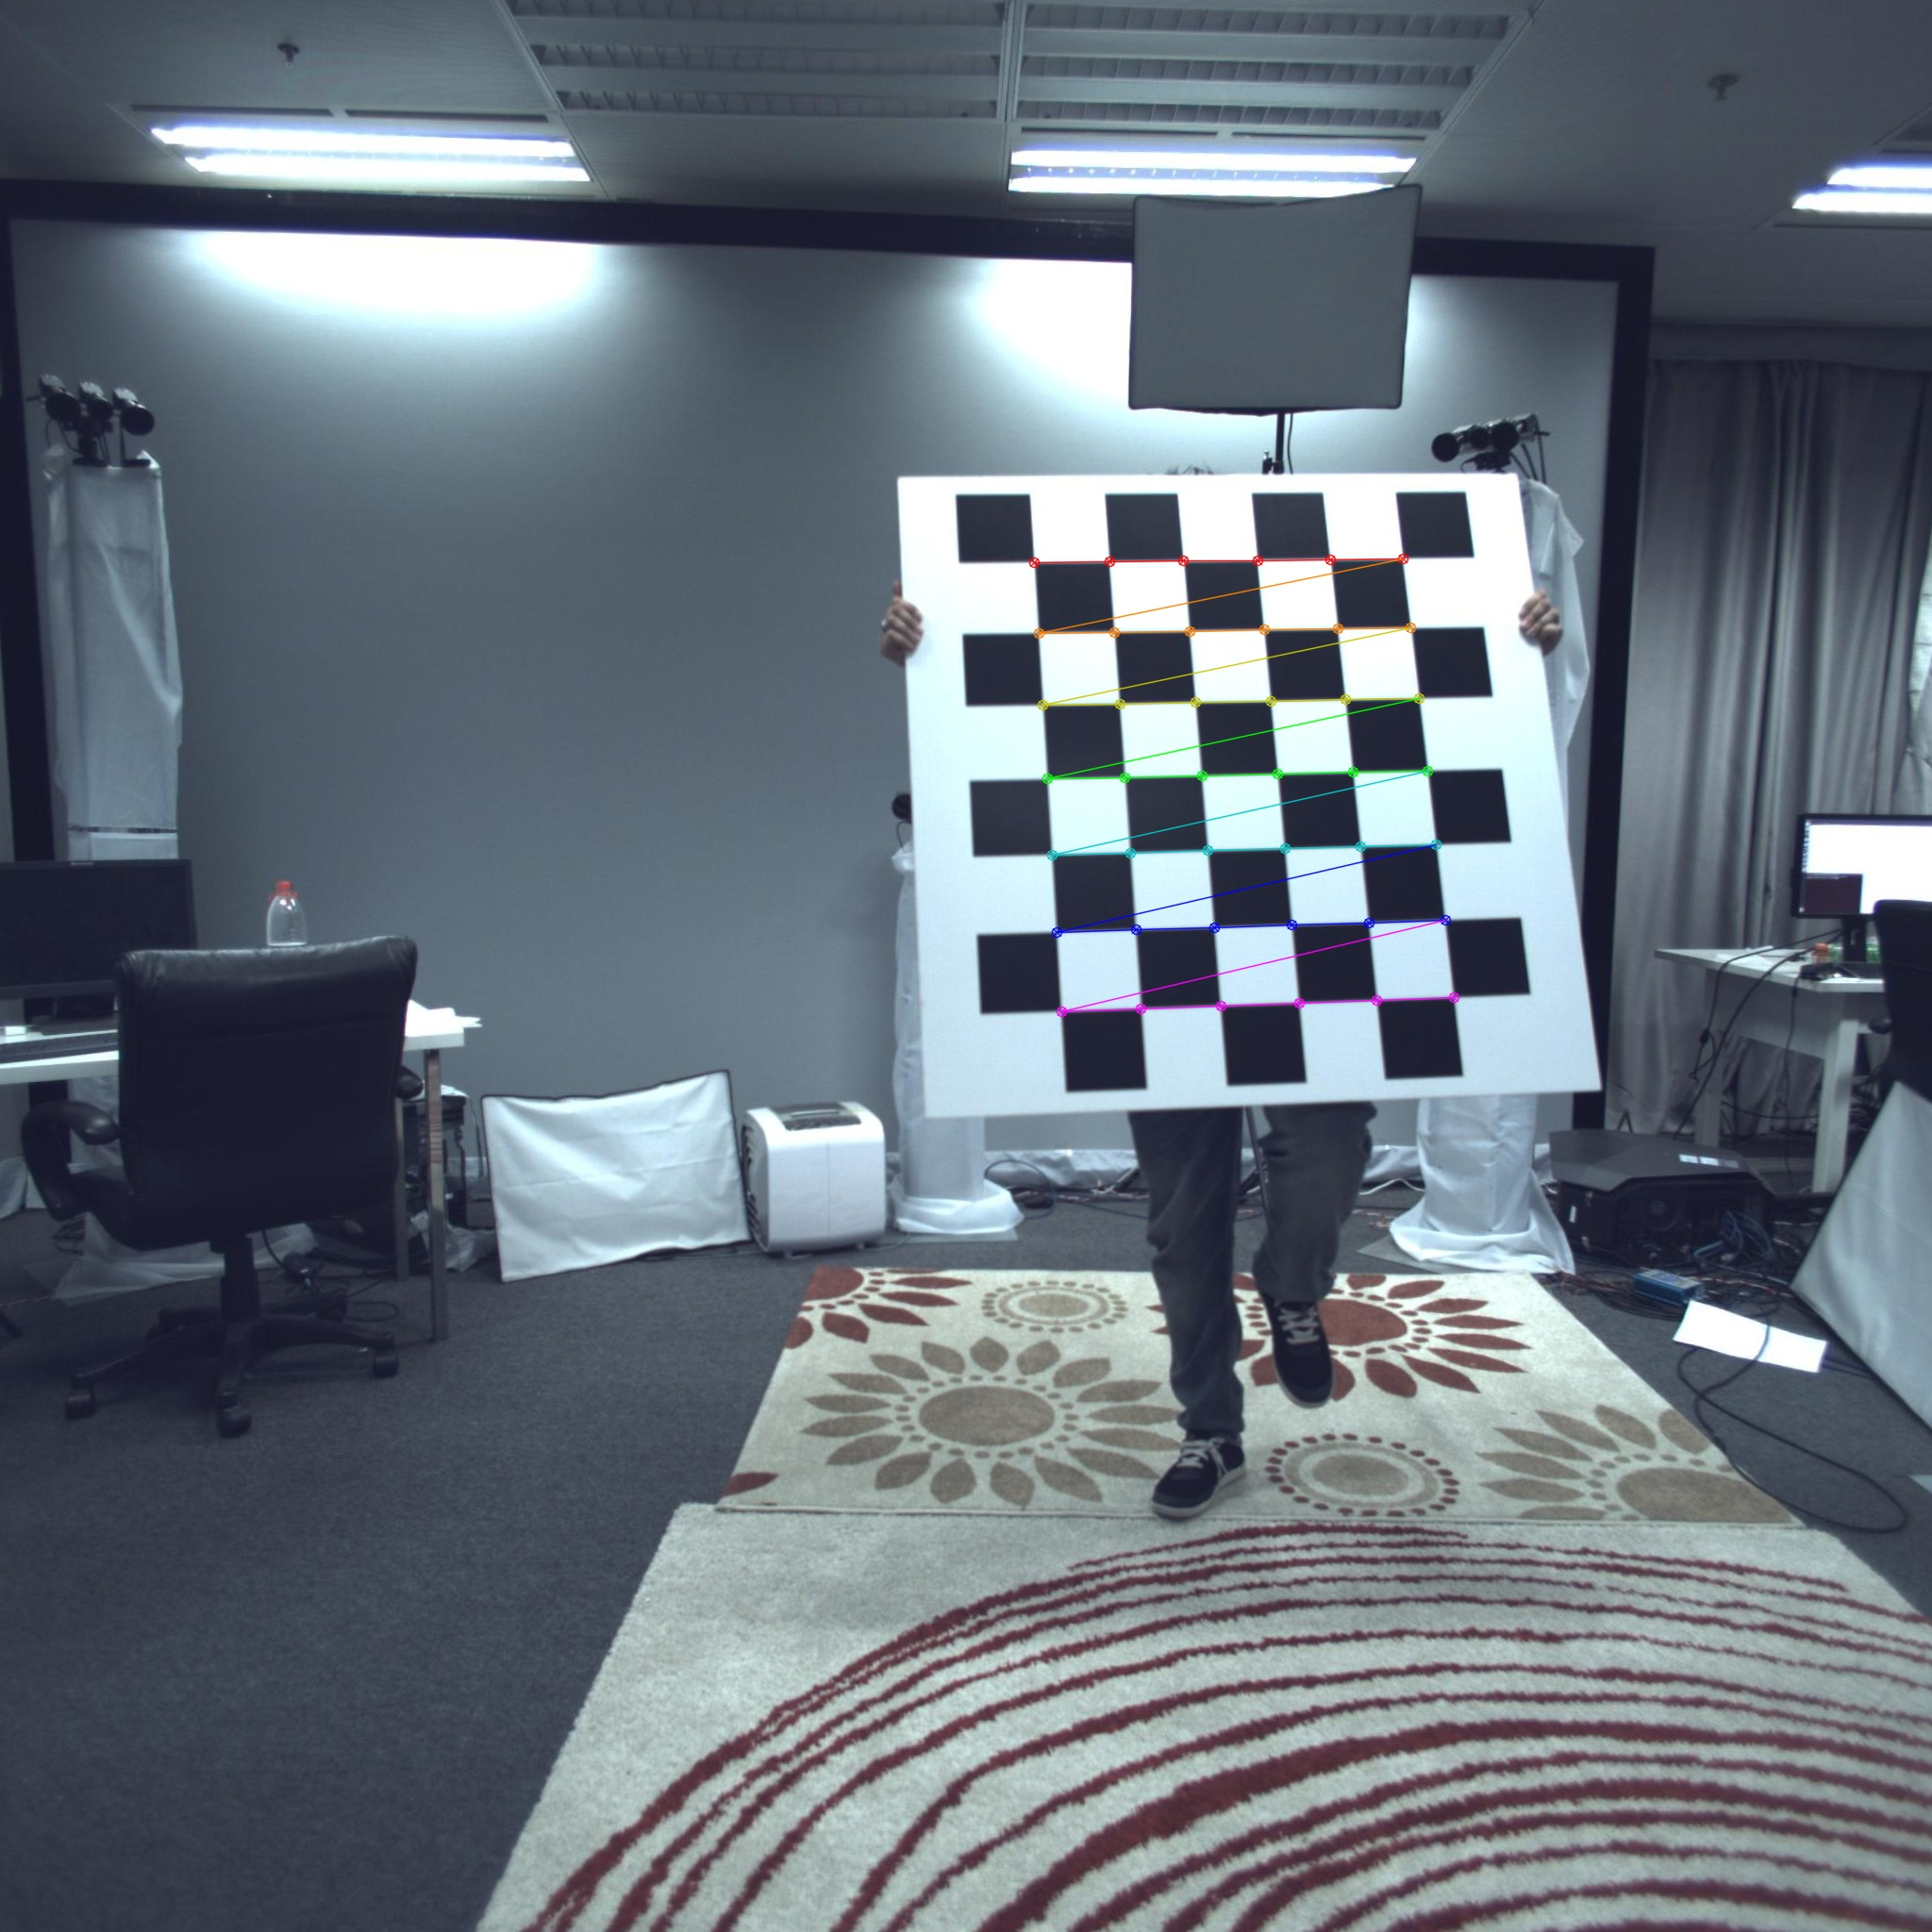
\includegraphics[scale=0.058]{image/free.jpg}
  \vspace{0cm}
  \centerline{(a)}\medskip
\end{minipage}
\hfill
\begin{minipage}[b]{0.48\linewidth}
  \centering
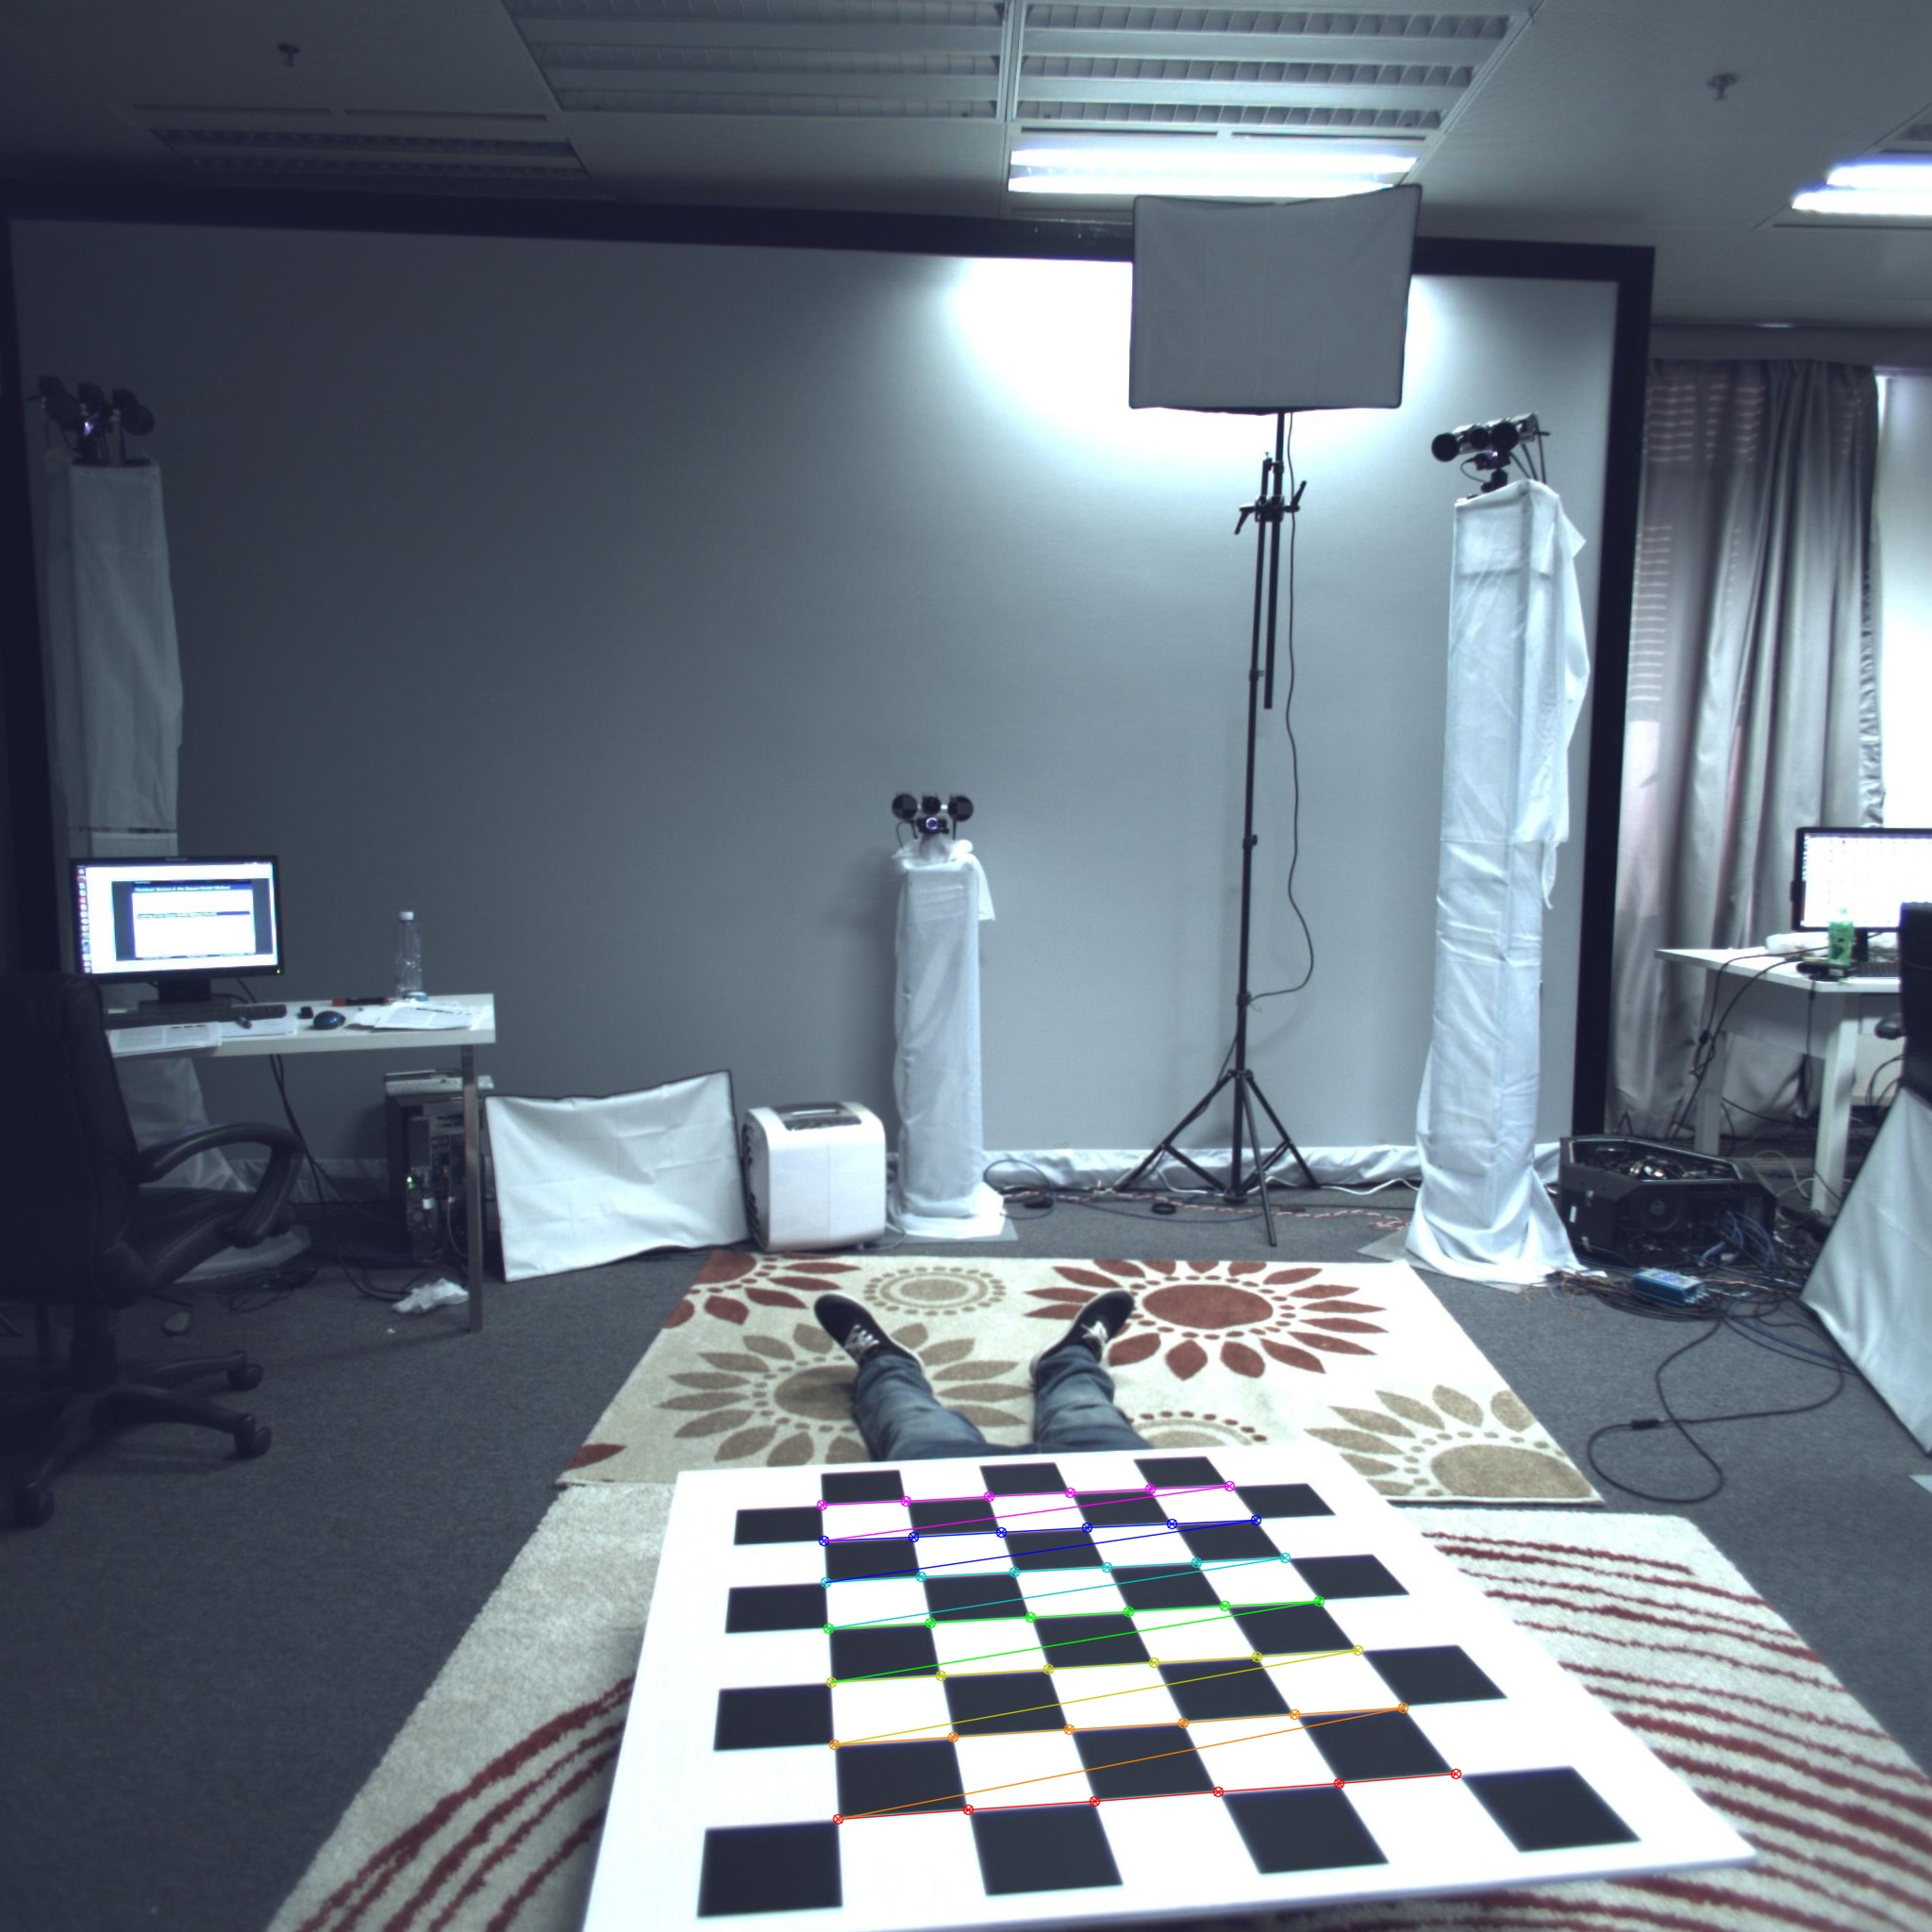
\includegraphics[scale=0.058]{image/ground.jpg}
  \vspace{0cm}
  \centerline{(b)}\medskip
\end{minipage}
%
\caption{Results of the checkerboard corners detection. (a): Results when the user moves freely. (b): Results when the checkerboard is on the ground. }
\label{fig:checkerboard}
\end{figure}



\section{point cloud registration}
\label{sec:registration}

We achieve the depth data from the 2 NIR cameras using depth estimation methods~\cite{Bleyer2011PatchMatch}. Although after the global optimization, we can get a result with less reprojection error, but it may not be the optimal solution to the 3D reconstruction because the quality of depth estimation also influence the final result. If the depth and camera parameters are both accurate enough, the point clouds of different views should align very well. 
However, the error cannot be avoided completely.
\xj{what error? caused by what?}

We reconstruct the point cloud of one view using the depth data, found the distortion on the boundary of the model, especially near the head, as shown in Figure~\ref{fig:deptherror}. Moreover, although the reprojection error after the global optimization mentioned in the last section is at sub-pixel level, we also find the separation between the point cloud of different views, effecting the quality of reconstruction. 
%
To minimize the error from depth data and achieve high-quality reconstruction results, we use ICP to map the inaccurate depth to a 3D model by point cloud registration.
\begin{figure}[ht]
\centering
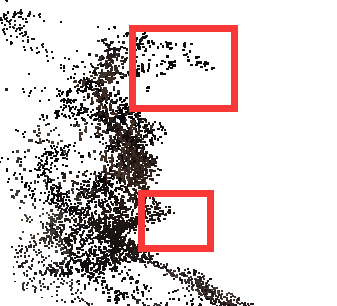
\includegraphics[scale=0.4]{image/depth_error.png}
\caption{The distortion near the head of the model of a single view which is caused by the inaccurate depth estimation. \xj{It is not clear. show a rgb image? or depth map from the camera view?}}
\label{fig:deptherror}
\end{figure}



For each point reconstructed by the depth image, we consider an estimation
\begin{equation}
\mathbf{\tilde{P}}_{ij}=f_{i}(\mathbf{P}_{j}),
\end{equation}
where $\mathbf{P}_{j}$ is the true 3D coordinates in the camera coordinate system. $f_{i}$ is a nonlinear function for view $i$, represent the depth influence. $\mathbf{\tilde{P}}_{ij}$ is the 3D coordinates we get from the depth data and intrinsic parameters in view $i$. With the extrinsic parameter, we can transform all the points into the world coordinate system. The estimation can be written as
\begin{equation}
\mathbf{\hat{P}}_{gj}=g(\mathbf{K_{ex}}_{i})f_{i}(\mathbf{P}_{j}),
\end{equation}
where $\mathbf{\hat{P}}_{gj}$ is the 3D coordinates in the world coordinate system we reconstruct from the depth and camera parameters. ICP can be replaced as a rigid transform to all views
\begin{equation}
\mathbf{\tilde{\hat{P}}}_{gj}=M_{i}g(\mathbf{K_{ex}}_{i})f_{i}(\mathbf{P}_{j})=g(\mathbf{K_{ex}}_{i})M_{i}f_{i}(\mathbf{P}_{j}),
\end{equation}
where $\mathbf{\tilde{\hat{P}}}_{gj}$ is the coordinates of the point after the alignment. The transform $M_{i}$ can refine the error caused by $f_{i}$, and improve the quality of the result of 3D reconstruction.

We choose the point cloud of view 1 as the reference, align the point cloud of view 2 to it, combine the result of the two views, then align the point cloud of view 3 to the combined result and so on. Each ICP process produce a transformation matrix, then we can map the inaccurate depth to a high-quality 3D model using the rigid transformation.


\xj{Show depth maps from 8 views. Show three fused models from pairwisely estimated camera parameters, globally estimated camera parameters, and after icp registration.  }


% References should be produced using the bibtex program from suitable
% BiBTeX files (here: strings, refs, manuals). The IEEEbib.bst bibliography
% style file from IEEE produces unsorted bibliography list.
% -------------------------------------------------------------------------
 

\subsection{Point cloud registration}
\label{sec:registration}


%We achieve the depth data from the 2 NIR cameras using depth estimation methods~\cite{Bleyer2011PatchMatch}.
After the global optimization, we get a set of camera parameters with the minimal re-projection error.
However, there are still many problems in the 3D model obtained from directly merging the partial point clouds estimated from different views according to the estimated camera poses, mainly due to the low quality of depth estimation.
%
%If the depth and camera parameters are both accurate enough, the point clouds of different views should align very well.
%
While our global calibration step provides highly accurate camera poses, the point clouds from neighboring camera pods are close to each other in a coarse level.
The misalignment typically occurs at some parts of the human body, such as the head and arms, due to the depth estimation error in theses regions.
%
Therefore, we use the Iterative Closest Point (ICP) algorithm~\cite{Besl1992A} to slightly adjust the rigid transformation between two partial point clouds, and fuse the transformed point clouds to balance out the depth errors.
%

We choose the point cloud of one view as the reference, and compute the transformation of the point clouds from its neighboring views to it using the ICP algorithm. 
We then merge the point clouds as a new reference. 
The other views are registered sequentially in a similar way. 
When all the point clouds of different views are registered, a high-quality 3D model can be achieved, as shown in Fig.~\ref{fig:3Dmodel}.
\begin{figure}[ht]
%
\begin{minipage}[b]{.48\linewidth}
  \centering
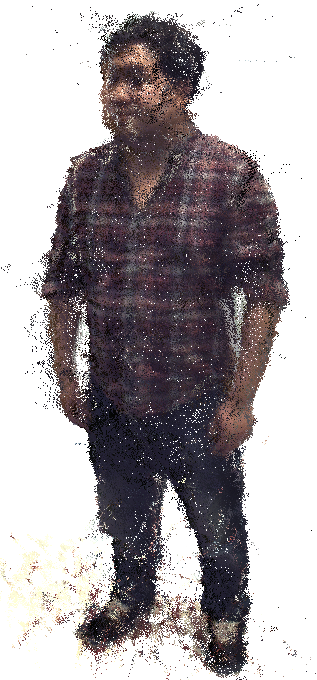
\includegraphics[width=3.cm]{image/model_front.png}
  \vspace{0cm}
  \centerline{(a)}\medskip
\end{minipage}
\hfill
\begin{minipage}[b]{0.48\linewidth}
  \centering
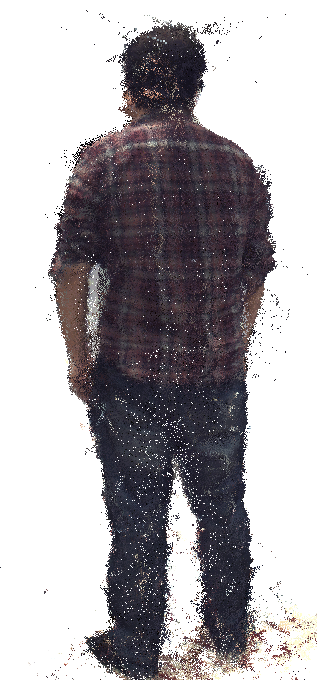
\includegraphics[width=3.cm]{image/model_back.png}
  \vspace{0cm}
  \centerline{(b)}\medskip
\end{minipage}
%
\caption{An 3D model after ICP registration. (a) The front side of the model. (b) The back side of the model. }
\label{fig:3Dmodel}
\end{figure}


\comments{
Most depth-estimation techniques based on NIR cameras are not robust enough, especially for light-absorbing materials like black hair.
Moreover, the depth estimation may be affected by many factors like the quality of the laser pointer, the interaction effect on the camera pods which are arranged towards each other caused by the laser and similarity.
%Although there have been many research on it, the error cannot be avoided completely.
As Fig.~\ref{fig:deptherror} shows, the estimated depth encounters large distortions on the boundary of the human body, and missing data in the head area.
Directly merge the point clouds estimated from 8 views according to the estimated camera parameters leads to a noisy and distorted point cloud, as Fig.~\ref{fig:} (a)(b) shows.\md{ToDo}


The point clouds reconstructed from different views are quite close to each other because of the global calibration, hence there is no need for the coarse registration.
We tried the state-of-the-art global registration algorithms~\cite{Evangelidis-ECCV-2014} to register all the point clouds from different views simultaneously without the corresponding points. However, the point clouds produced by our multi-camera system may have no overlapping fields, which leads to the wrong results. For example, the point cloud of the back of a human body may be aligned to the front overlappingly because of the symmetry of the shape of the body. To avoid these kinds of mistakes, we register the point clouds in multi views sequentially.
}

\comments{
In this registration step, we \emph{fuse} the partial point clouds reconstructed from each view using the
We choose the point cloud of one view as the reference, and align the point cloud of its neighboring views sequentially, using the Iterative Closest Point algorithm. \xj{Add the reference. If do not considering the time, why don't you use other state-of-the-art algorithms?}
The registration step is to minimize the distance between the corresponding points in different views mainly caused by the depth maps, which can be defined as:
\begin{equation}
E(\mathbf{R},\mathbf{T})=\sum_{N}(\mathbf{P}_{t}-\mathbf{R}\times\mathbf{P}_{s}-\mathbf{T})^{2},
\end{equation}
where $\mathbf{P}_{t}$ and $\mathbf{P}_{s}$ are a pair of corresponding points in the point clouds of the two views, N is the total number of the corresponding points, $\mathbf{R}$ and $\mathbf{T}$ represents the rigid transform, $\mathbf{R}$ is the rotation matrix and $\mathbf{T}$ is the translation matrix.

After the registration step, the point cloud which are not aligned very well because of the depth maps can be registered and a high-quality 3D model can be achieved.


Moreover, although the reprojection error after the global optimization mentioned in the last section is at sub-pixel level, which can prove the high accuracy of our calibration result, we still find the separation between the point cloud of different views when we map the depth to the entire model, effecting the quality of reconstruction. These deficiencies are mainly caused by the depth estimation.




To achieve a high-quality reconstruction, we fuse partial point clouds which are inaccurate and incomplete into a 3D model in a registration manner.
%
For each point reconstructed by the depth image, we consider an estimation.
\begin{equation}
\mathbf{\tilde{P}}_{ij}=f_{i}(\mathbf{P}_{j}),
\end{equation}
where $\mathbf{P}_{j}$ is the true 3D coordinates in the camera coordinate system. $f_{i}$ is a nonlinear function for view $i$, represent the depth influence. $\mathbf{\tilde{P}}_{ij}$ is the 3D coordinates we get from the depth data and intrinsic parameters in view $i$. With the extrinsic parameter, we can transform all the points into the world coordinate system. The estimation can be written as
\begin{equation}
\mathbf{\hat{P}}_{gj}=g(\mathbf{K_{ex}}_{i})f_{i}(\mathbf{P}_{j}),
\end{equation}
where $\mathbf{\hat{P}}_{gj}$ is the 3D coordinates in the world coordinate system we reconstruct from the depth and camera parameters. ICP can be replaced as a rigid transform to all views
\begin{equation}
\mathbf{\tilde{\hat{P}}}_{gj}=M_{i}g(\mathbf{K_{ex}}_{i})f_{i}(\mathbf{P}_{j})=g(\mathbf{K_{ex}}_{i})M_{i}f_{i}(\mathbf{P}_{j}),
\end{equation}
where $\mathbf{\tilde{\hat{P}}}_{gj}$ is the coordinates of the point after the alignment. The transform $M_{i}$ can refine the error caused by $f_{i}$, and improve the quality of the result of 3D reconstruction.
}%

% view 2 to it, combine the result of the two views, then align the point cloud of view 3 to the combined result and so on.
%Each ICP process produce a transformation matrix, then we can map the inaccurate depth to a high-quality 3D model using the rigid transformation.




\section{Results and Discussion}
\label{sec:Results}

In order to evaluate the impacts of different components of our hybrid system, a series of experiments are conducted. We first show the re-projection error of different methods. Then we quantitatively analyze the reconstruction quality using a ground-truth model scanned by an accurate Lidar scanner.  
Finally we show the reconstructed models of human bodies under different pose to demonstrate the robustness of our method.

\xj{Discussion on time.}

\noindent\textbf{Camera Calibration Accuracy.} 
%
The re-projection error describes the accuracy of the calibration system. 
We compute the re-projection and compare it to evaluate the effectiveness of our global calibration step.
%
Using the 2D coordinates of the corners detected in the checkerboard images, we can achieve the 3D space coordinates $\mathbf{P_{c}}$ by triangulation \xj{using what camera parameters?}. 
Then we re-project $\mathbf{P_{c}}$ to each view which the checkerboard can be seen using the extrinsic parameters obtained by different methods and compute the average re-projection error, as shown in Table~\ref{tab:reprojection}.


\begin{table*}
	\centering
	\caption{Average re-projection error (pixels) of each camera using different methods. (a) results by Kalibr~\cite{Maye2013Self}, (b) results by Kalibr ~\cite{Maye2013Self} with our registration step, (c) results by our global calibration method, (d) results by our integrated method. The re-projection error of (c) is the smaller and uniform in each view, while the results of other methods contain the accumulative error and the inconsistence. }
	\label{tab:reprojection}
	\begin{tabular}{lcccccccc}
		\hline
		Methods & Cam 1 & Cam 2 & Cam 3 & Cam 4 & Cam 5 & Cam 6 & Cam 7 & Cam 8\\
		\hline
		(a) Kalibr &4.54 &3.20 &11.16 &10.74 &4.87 &6.75 &3.64 &5.11\\

		(b) Kalibr+ICP &3.75 &4.04 &11.40 &7.91 &6.39 &5.62 &3.39 &5.74\\
		
		(c) SBA   &\textbf{0.32} &\textbf{0.32} &\textbf{0.38}  &\textbf{0.35} &\textbf{0.37} &\textbf{0.40} &\textbf{0.33} &\textbf{0.34} \\
		
		(d) SBA+ICP &0.92 &0.99 &1.58 &2.19 &3.06 &1.79 &2.68 &1.38\\
		\hline
		
	\end{tabular}


\end{table*}


The reprojection error of the proposed global calibration method is the smaller \xj{smallest?} among different methods, which proves that the global optimization is quite effective. 
Although the registration step makes the model closer to the ground truth, it leads to bigger reprojection error. That is because the aim of the registration step is to minimize the error caused by the inaccurate depth estimation, but not to optimize the camera parameters.


\noindent\textbf{Reconstruction Quality.}
%\xj{Explain why do you need this experiment.}
The final goal of our system is to achieve a high-quality reconstruction model, we quantitatively compare the results reconstructed by different methods.
%
We generate a ground-truth model by scanning a plaster model of a human head using a 3D laser scanner with the scanning error smaller than 0.04 mm \xj{in what depth range?}. 
%
The model is placed in the center of our multi-camera system and the RGB and depth images of it can be obtained. \xj{how do you know where is the center? }
%We consider the accurate mesh as the ground truth and compare it with the reconstructed 3D model using different methods.
We compute the L2 distances of the fused point clouds to the ground-truth mesh for different variants of our method. 
For each point $\vb{p}$ in the reconstructed point cloud, we search for its nearest point $\vb{q}$ on the mesh, and compute the distance $\|\vb{p}-\vb{q}\|$. 
%
The average error is listed in Table~\ref{fig:distance}. \xj{show a chart?} 
As we can see, the reconstructed model combining SBA and registration has the smallest error, which proves that it can achieve a high-quality model.
We also show the distribution histogram of the error using different extrinsic parameters in Figure~\ref{fig:histogram}. 
Similarly, the result of our method has the most accurate result.
\xj{Combine the distribution figure with table as two charts.}

\begin{figure*}[ht]
  \centering
\subfigure[]{
\begin{minipage}[c]{.22\linewidth}
\centering
  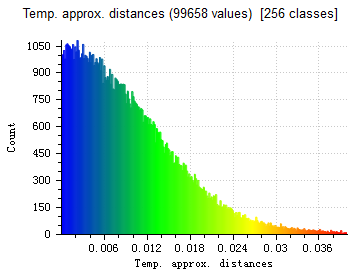
\includegraphics[width=4cm]{image/dis_1.png}
\end{minipage}
}%
\subfigure[]{
\begin{minipage}[c]{.22\linewidth}
\centering
  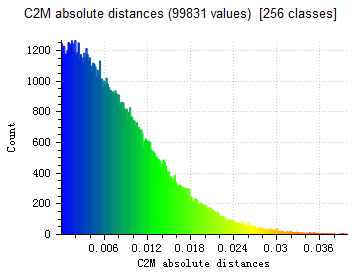
\includegraphics[width=4cm]{image/dis_2.png}
\end{minipage}
}
\subfigure[]{
\begin{minipage}[c]{.22\linewidth}
\centering
  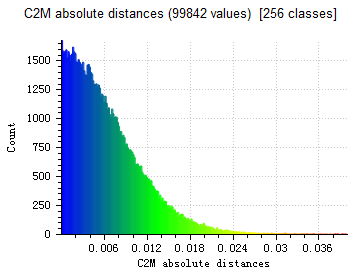
\includegraphics[width=4cm]{image/dis_3.png}
\end{minipage}
}
\subfigure[]{
\begin{minipage}[c]{.22\linewidth}
\centering
  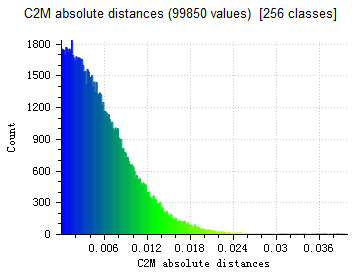
\includegraphics[width=4cm]{image/dis_4.png}
\end{minipage}
}
\caption{The distribution histogram of the L2 distances of the point cloud reconstructed using different methods to the ground truth. (a) results by Kalibr ~\cite{Maye2013Self}, (b) results by Kalibr ~\cite{Maye2013Self} with our registration step, (c) results by our global calibration method, (d) results by our integrated method. The number of the points with small distance increases obviously after the optimization and registration step we proposed.}
\label{fig:histogram}
\end{figure*}

\noindent \textbf{More Reconstructed Models.}
%
We reconstruct the 3D point clouds of a human body standing in the center of our multi-camera system using various methods.  We mark the point cloud in different views with different colors to show the quality of the fusion results. Figure~\ref{fig:pointcloud} shows the results which demonstrate our algorithm. As we can see, the model reconstructed by our hybrid system has the highest quality. 

\xj{Show at least three groups of results, in different human pose.}

\begin{figure*}[ht]
  \centering
\subfigure[]{
\begin{minipage}[c]{.22\linewidth}
\centering
  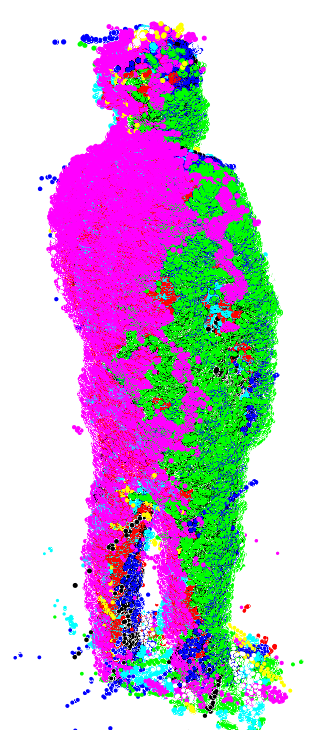
\includegraphics[width=2.5cm]{image/pc_1.png}
\end{minipage}
}%
\subfigure[]{
\begin{minipage}[c]{.22\linewidth}
\centering
  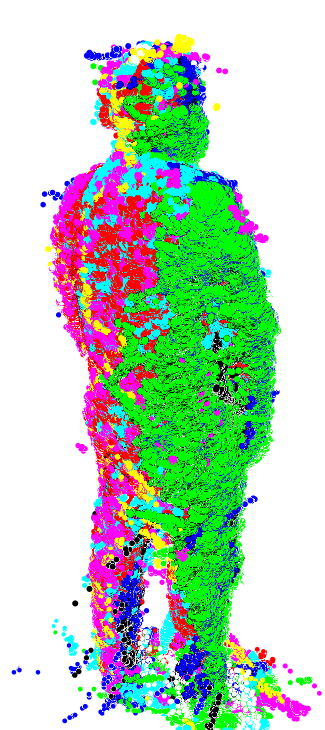
\includegraphics[width=2.5cm]{image/pc_2.png}
\end{minipage}
}
\subfigure[]{
\begin{minipage}[c]{.22\linewidth}
\centering
  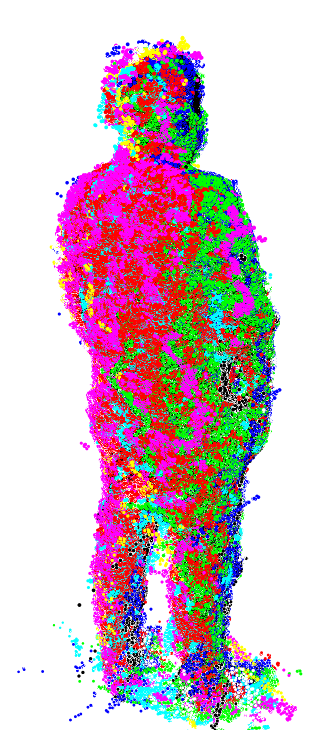
\includegraphics[width=2.5cm]{image/pc_3.png}
\end{minipage}
}
\subfigure[]{
\begin{minipage}[c]{.22\linewidth}
\centering
  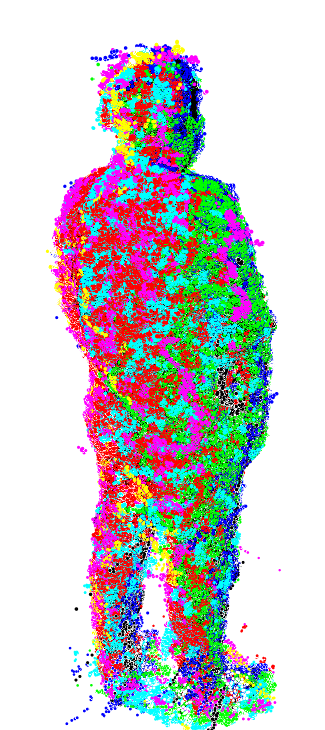
\includegraphics[width=2.5cm]{image/pc_4.png}
\end{minipage}
}
\caption{The reconstruction results of the back of a human using various methods.(a) results by Kalibr ~\cite{Maye2013Self}, (b) results by Kalibr ~\cite{Maye2013Self} with our registration step, (c) results by our global calibration method, (d) results by our integrated method. We render the point clouds with different colors to distinguish which view the point clouds belong to. The point clouds in result (a) are distinctly separated from other views, as the pink and green views cover the whole surface of the model. Result (b) becomes a little better while the green view still covers the right side of the body. The point clouds align quite well in result (c) with small blemishes, the azure view is inside the model. (d) shows a well-aligned model. }
\label{fig:pointcloud}
\end{figure*}


\begin{figure*}[ht]
  \centering
\subfigure[]{
\begin{minipage}[c]{.22\linewidth}
\centering
  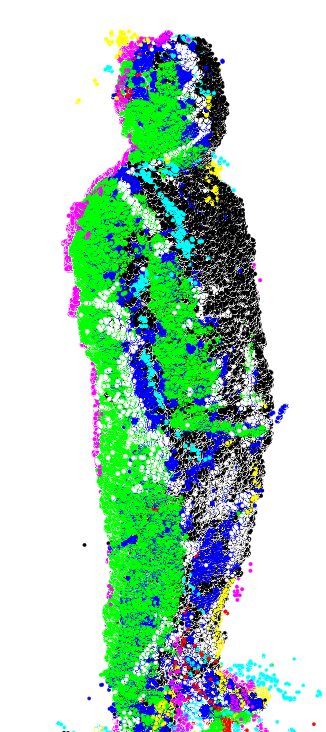
\includegraphics[width=2.5cm]{image/pc_1_1.png}
\end{minipage}
}%
\subfigure[]{
\begin{minipage}[c]{.22\linewidth}
\centering
  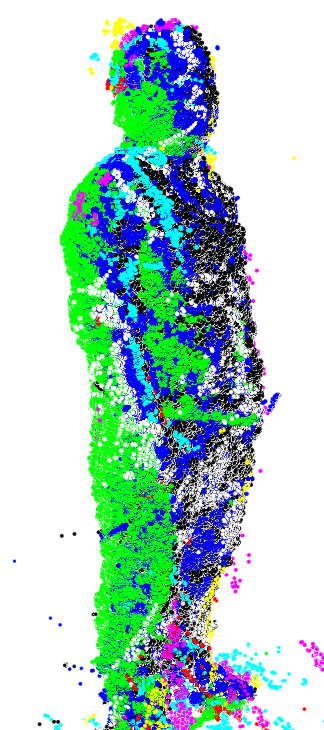
\includegraphics[width=2.5cm]{image/pc_2_1.png}
\end{minipage}
}
\subfigure[]{
\begin{minipage}[c]{.22\linewidth}
\centering
  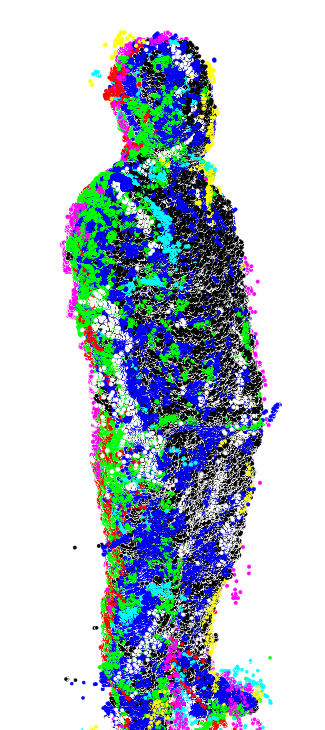
\includegraphics[width=2.5cm]{image/pc_3_1.png}
\end{minipage}
}
\subfigure[]{
\begin{minipage}[c]{.22\linewidth}
\centering
  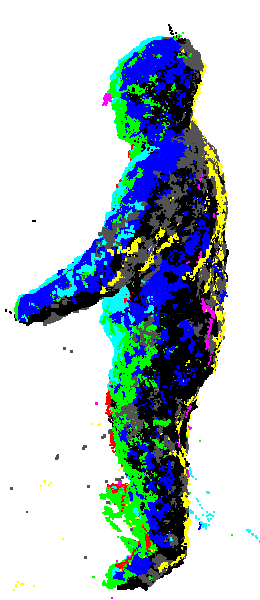
\includegraphics[width=2.5cm]{image/pc_4_1.png}
\end{minipage}
}
\caption{The reconstruction results of the back of a human using various methods.(a) results by Kalibr ~\cite{Maye2013Self}, (b) results by Kalibr ~\cite{Maye2013Self} with our registration step, (c) results by our global calibration method, (d) results by our integrated method.}
\label{fig:pointcloud}
\end{figure*}

\begin{figure*}[ht]
  \centering
\subfigure[]{
\begin{minipage}[c]{.22\linewidth}
\centering
  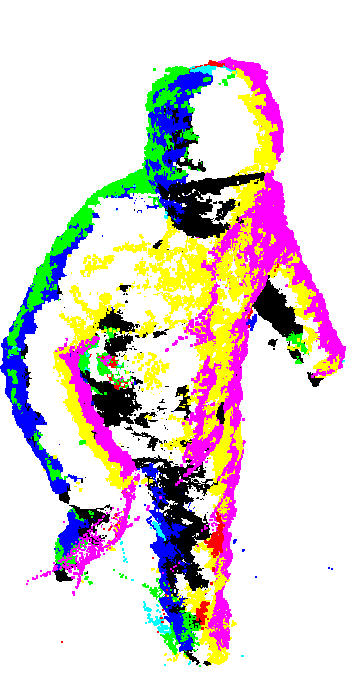
\includegraphics[width=2.5cm]{image/pc_1_2.png}
\end{minipage}
}%
\subfigure[]{
\begin{minipage}[c]{.22\linewidth}
\centering
  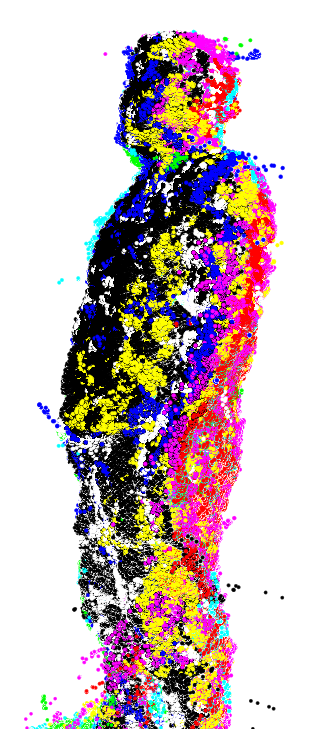
\includegraphics[width=2.5cm]{image/pc_2_2.png}
\end{minipage}
}
\subfigure[]{
\begin{minipage}[c]{.22\linewidth}
\centering
  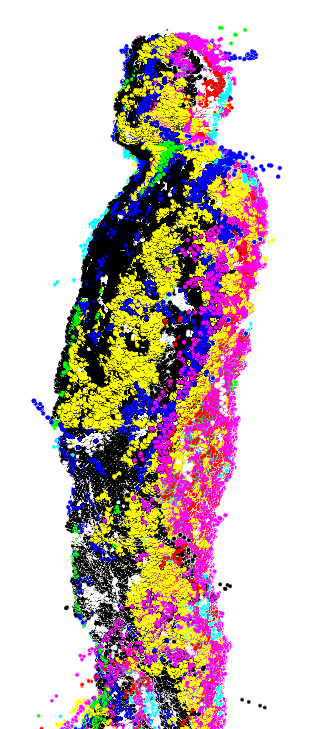
\includegraphics[width=2.5cm]{image/pc_3_2.png}
\end{minipage}
}
\subfigure[]{
\begin{minipage}[c]{.22\linewidth}
\centering
  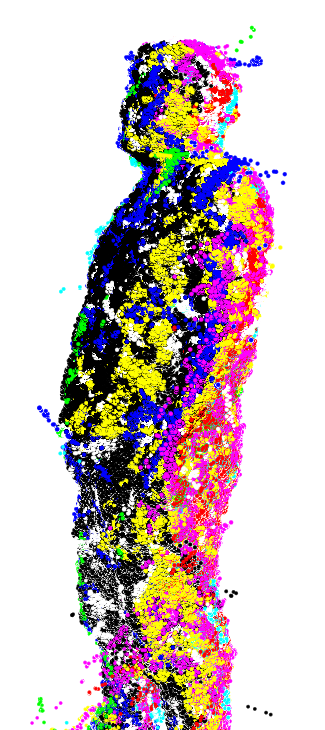
\includegraphics[width=2.5cm]{image/pc_4_2.png}
\end{minipage}
}
\caption{The reconstruction results of the back of a human using various methods.(a) results by Kalibr ~\cite{Maye2013Self}, (b) results by Kalibr ~\cite{Maye2013Self} with our registration step, (c) results by our global calibration method, (d) results by our integrated method.}
\label{fig:pointcloud}
\end{figure*}
\section{conclusion}
We present an efficient system integrating the multi-camera calibration and point cloud registration. By a global bundle adjustment, we reduce the accumulative error and the inconsistence caused by the pairwise camera pose estimation, and achieve a set of accurate extrinsic parameters with less reprojection error. With the point cloud registration, we minimize the error from the depth estimation and achieve a high-quality 3D model. Our calibration algorithm has been tested on both reprojection error and ground truth data. The experimental results has proved that the two steps of our system are both necessary and effective, and a more accuracy model can be reconstructed using our method.
\begin{table}
	\centering
	\caption{The distance between the point cloud and the ground truth. The distance (in centimeters )of the point cloud to the mesh of the plaster model computed by four different methods. (a) results by Kalibr ~\cite{Maye2013Self}, (b) results by Kalibr ~\cite{Maye2013Self} with our registration step, (c) results by our global calibration method, (d) results by our integrated method.}
	\label{tab:distance}
	\begin{tabular}{lcccc}
		\hline
		Methods & Mean &Standard deviation\\
		\hline
		(a) &0.9542 &0.7240\\

		(b) &0.8243 &0.6376\\
		
		(c) &0.6408 &0.5072\\
		
		(d) &0.5811 &0.4650\\
		\hline
		
	\end{tabular}
\label{fig:distance}
\end{table}






% References should be produced using the bibtex program from suitable
% BiBTeX files (here: strings, refs, manuals). The IEEEbib.bst bibliography
% style file from IEEE produces unsorted bibliography list.
% -------------------------------------------------------------------------
\bibliographystyle{IEEEbib}
\bibliography{icme2018template}

\end{document}
